\chapter{Mobile Apps}
\label{mobileapps}
\index{Mobile Apps}
\index{Android App}
\index{IOS App}
\index{Mobile}


Accessing the Smart Home from a mobile device such as a phone or an iPad has become popular. 
\zway offers multiple ways to access a user interface from one of these 
mobile devices. Thanks to an open API, it is also possible to design your mobile app or 
use third-party apps supporting \zway.

Hence, while other vendors offer just one app per mobile platform (Android, IOS), \zway 
allows you to choose what you like best.

\section{Standard mobile web browsers}

\begin{figure}
\begin{center}
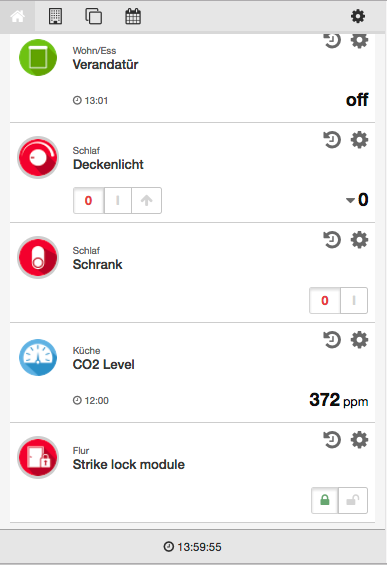
\includegraphics[width=0.4\textwidth]{pngs/cap5/mobile1.png}
\caption{Web User Interface on small mobile screen}
\label{mobile1}
\end{center}
\end{figure}

The \zwshui and the \zweui are developed as a responsive design, meaning that the web 
pages will determine the screen size of your device and re-render accordingly.
As a result, the \zwshui and the \zweui described 
in Chapter \ref{eui} are quite usable with small mobile screens. Figure \ref{mobile1} 
shows a dialog from the web browser interface on a small mobile screen.

The \zwshui will always be the most advanced and most recent interface 
incorporating all new functions and features. This means accessing the user interface 
on a mobile device with a standard browser makes these functions available on the 
mobile device first.

The big disadvantage is that the interface is certainly slower than a native app, and the 
dialogs and menu items may only be partly optimized for small screens.

Accessing the user interface from a mobile web browser is not much different than from a 
PC-based browser. Just type in the IP address of the controller or use the find.zwave.me service.

\section{Native HTML based apps}

\begin{figure}
\begin{center}
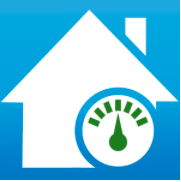
\includegraphics[width=0.2\textwidth]{pngs/cap5/mobile2.png}
\caption{Mobile App Icon from App Store}
\label{mobile2}
\end{center}
\end{figure}

It is interesting that most apps available in the commonly used app stores are written 
in HTML and embedded into a native wrapper that allows enhancing the HTMP pages with 
further functions. The standard \zway apps in the iTunes and Google Play Store follow 
this approach. You find the apps here:

\begin{itemize}
\item Android: https://play.google.com/store/apps/details? id=com.app.zwave.zway\_control
\item IOS: https://itunes.apple.com/de/app/zway-control/id1033129180
\end{itemize}


\begin{figure}
\begin{center}
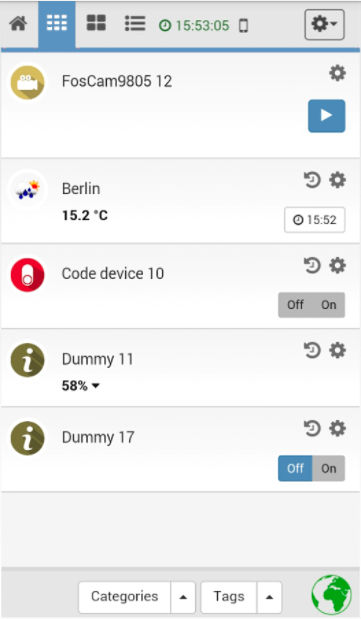
\includegraphics[width=0.3\textwidth]{pngs/cap5/mobile3.png}
\caption{Native HTML based app}
\label{mobile3}
\end{center}
\end{figure}

The apps are optimized for mobile devices and apps, e.g. to use the QR code for a fast 
setup. They will also cache data better and align some other functions.
There is only one drawback. If the app is used for inhouse control, such fast access to 
lights, the overall design of the data handling and caching will still imply some delays. 
Also, the app only allows managing one home per device since it cannot be installed twice 
for two different homes.

\section{Pure Native Apps}

For the Android platform only, there is a second \zway control app that is written 
completely in Java for very fast access to actuators. The usage philosophy is similar to 
the other apps with dashboard, room view, timeline, history, etc. Figure \ref{mobile3} 
gives one view of the app.

\begin{figure}
\begin{center}
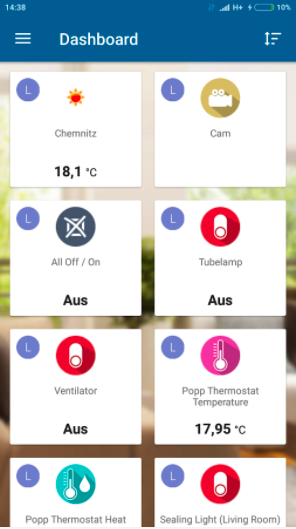
\includegraphics[width=0.3\textwidth]{pngs/cap5/mobile5.png}
\caption{Native fast app for Android}
\label{mobile5}
\end{center}
\end{figure}

The app, named \app{Z-Way Control}, is available on the Google Play Store:

\begin{itemize}
\item https://play.google.com/store/apps/details?id=de.pathec.hubapp\&hl=de
\end{itemize}

\section{Third-Party Apps}

The outstanding reputation of \zway as \zwave backend caused many third-party suppliers 
and developers to support \zway with their frontends. The following explanations can only 
cover a subset of solution and user interfaces. However, the three examples show three 
very typical approaches.

\subsection{Imperihome}
\index{Imperihome}

Imperihome is a vendor-agnostic app that is available for various mobile platforms. It 
supports quite a long list of smart home devices and systems such as \zway. The basic 
version of the app is available free of cost. The extended version costs some 5 USD/EUR.

\begin{figure}
\begin{center}
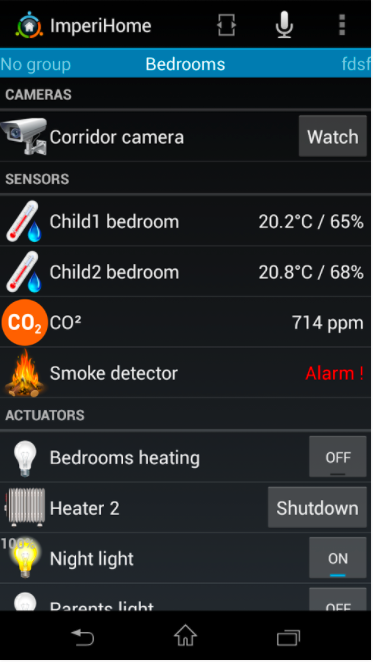
\includegraphics[width=0.4\textwidth]{pngs/cap5/mobile4.png}
\caption{Imperihome App}
\label{mobile4}
\end{center}
\end{figure}

\subsection{Fibaro}
\index{Fibaro}

\begin{figure}
\begin{center}
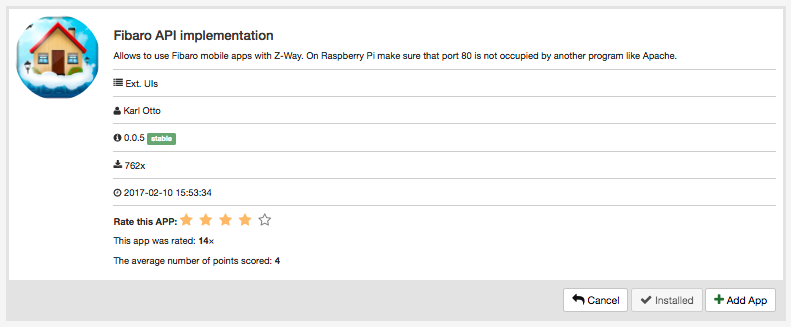
\includegraphics[width=0.4\textwidth]{pngs/cap5/mobile6.png}
\caption{\zway app to support Fibaro Mobile App}
\label{mobile6}
\end{center}
\end{figure}

Fibaro is one of the leading \zwave-based smart home suppliers in Europe. They offer their 
own \zwave smart home controller, Home Centre Lite of Home Centre 2. Fibaro is focused on 
design and so their mobile app is quite stylish too.

You can use the Fibaro app, which is designed for their own Home Centre 2, to control 
\zway.

\begin{figure}
\begin{center}
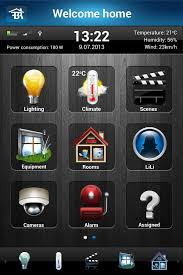
\includegraphics[width=0.4\textwidth]{pngs/cap5/mobile8.jpeg}
\caption{Fibaro Mobile App}
\label{mobile8}
\end{center}
\end{figure}

Just download the Fibaro supporter app from the \zway app store. Chapter \ref{apps} 
describes how to do this. After that, download the Fibaro mobile app from iTunes or Google 
Play Store, and configure accordingly.

\subsection{openHAB}

openHAB (www.openhab.org) is one example of an open source smart home control system that 
uses \zway to manage the \zwave network part. Once the connection is set up, it is possible 
to use one of the mobile openHAB apps to control \zway-connected devices. For more information 
about this binding between \zway and openHAB, please refer to the openHAB website.
